\documentclass[twocolumn, a4j]{ltjsarticle}
\usepackage{graphicx}
\usepackage[colorlinks, linkcolor=blue, bookmarksnumbered]{hyperref}
\usepackage{siunitx}
\usepackage{amsmath}
\usepackage[nameinlink]{cleveref}
\usepackage[subrefformat=parens]{subcaption}
\usepackage[top=2.5cm, bottom=2.5cm, left=2cm, right=2cm]{geometry}

\newcommand{\Cite}[1]{$^{\cref{#1}}$}

\crefformat{section}{#2第#1章#3}
\crefformat{subsection}{#2第#1節#3}
\crefformat{enumi}{#2(#1)#3}
\crefname{figure}{図}{図}
\crefname{table}{表}{表}
\crefname{equation}{式}{式}
\newcommand{\crefrangeconjunction}{-}
\newcommand{\crefrangepreconjunction}{}
\newcommand{\crefrangepostconjunction}{}
\newcommand{\crefpairconjunction}{、}
\newcommand{\crefmiddleconjunction}{、}
\newcommand{\creflastconjunction}{、}
\newcommand{\crefpairgroupconjunction}{、}
\newcommand{\crefmiddlegroupconjunction}{、}
\newcommand{\creflastgroupconjunction}{、}

\sisetup{inter-unit-product=\ensuremath{{}\cdot{}}}
\newcommand{\SII}[2]{\SI{#1}{[#2]}}

\title{粒子法FLOSSに対する妥当性確認試験 \\ Validation for Particle Method FLOSS}

\author{吉藤尚生、大友広幸 \\
	株式会社フィックスターズ \\
	東京都品川区大崎1-11-1 \\
	E-mail:yoshifuji@fixstars.com}

\date{2019年10月28日(第33回数値流体力学シンポジウム向け原稿)}

\begin{document}
\maketitle

\begin{abstract}
We created three benchmark problems to validate FLOSS of the Particle Method.
The targets were DualSPHysics and OpenMPS, which are mainly aim to apply in coastal and ocean engineering.
The first benchmark, the Central Gravity problem, validates the hydrostatic pressure.
It found that DualSPHysics is not able to solve the hydrostatic problem due to its density formulation.
It also found that MPS-GC method causes nonphysical surface oscillation due to nonconservation of momentum.
The second and third benchmarks are based on the Dambreak problem.
They validate the time series of the surface shape, water depth, and pressure.
The benchmark results showed that MPS-SPP is necessary to reduce the pressure fluctuation.
We continue to develop and invoke verification and validation for Particle Method FLOSS.
\end{abstract}

\section{背景}
	古くから人類は、安全な社会を目指し技術を発展させてきた。
	特に、日本を含めた自然災害の多い国では、防災・減災が社会的に重要な課題となっている。
	そのような中で、数値流体力学を含めた計算機援用工学(CAE)は、近年、主に土木構造物などの建造物の設計に広く用いられるようになってきた。
	そのため、数値流体力学的手法の改善は、安全な人類社会の達成にとても重要である。
	
	構造物の設計に現在広く用いられている計算手法は、格子を必要とする格子法である。
	しかし、海岸工学などの自由表面の大変形を伴う流れ場においては、表面の精度良い追跡が難しい。
	そこで、最近では、ラグランジュ的に移動する計算点(粒子)を用いる粒子法の応用が受け入れられつつある。

	現在では、粒子法の商用ソルバーも多く提供されており、例えば、Particleworks\Cite{ref:particleworks}、Abaqus/Explicit\Cite{ref:abaqus}、MPS-RYUJIN\Cite{ref:ryujin}などがある。
	ゆえに、粒子法を用いた解析を実施したい時には、これらを用いることで、自作のプログラムを作る必要は必ずしもない。
	
	これらの商用ソルバーは、有識者の手厚い支援や安定した環境が期待できる一方で、実装の詳細な検証や問題にあわせた解法の修正適用が難しい。
	また、開発がベンダーである会社の独占となるために、開発の方向性が、利用者ら(コミュニティ)の望む方向と必ず一致する保証がない。
	特に、安全な構造物の設計に用いるという観点からは、ソルバーは設計手法の一部であり、その動作の詳細や原理を正確に把握し検証できないことは大きな欠点となる。
	そのような背景から、近年では、オープンソースかつフリーソフトウェア(Free/Libre and Open Source Software; FLOSS)であるCAEツールを用いる「オープンCAE」が注目されるようになってきた。

	オープンCAEにおいては、各種プログラム・ソフトウェアは利用者が自由に閲覧・検証・改変することができ、また開発者を含む利用者コミュニティが開発を主導するという点が、商用ソルバーに対する長所となる。
	一方で、多くの場合開発リソースが商用ソルバーほど潤沢ではなく、そのコード品質やサポート体制には劣る。
	特に、商用ソルバーであれば、商品として提供するために多くの時間をかけて検証や妥当性確認(Verification and Validation; V\&V)がなされているが、FLOSSではそれらが満足できるほど実施されているとは言い難い。

	そこで著者らは、安全な人類社会の実現のための1つの手段として、主に海岸・海洋工学分野における粒子法FLOSSの開発・利用促進を目指している。
	現在は、その一環として妥当性確認を中心とした精度の確認と改善を進めており、本研究は、その最初の成果を報告するものである。
	
	今回対象とした粒子法FLOSSはDualSPHysicsとOpenMPSである。これらソフトウェアおよび実装されている手法については\cref{sec:method}で概説する。
	この2つのFLOSSに対して、自由表面を伴う流れの妥当性確認を実施するため、静水圧問題と水柱崩壊問題という2種類の最も基礎的なベンチマークを設定した。
	ベンチマークの詳細は\cref{sec:benchmark}で説明する。
	そして、DualSPHysicsとOpenMPSに対してベンチマークを実行し妥当性確認を実施した結果を\cref{sec:result}で報告する。
	妥当性確認によって問題が発見されたため、それぞれその問題の原因追跡と解決法についても同節で結果と合わせて説明する。

\section{各ソフトウェアと実装されている手法 \label{sec:method}}
	今回対象とするソフトウェアは、どちらも非圧縮性流れニュートン流体のソルバーであり、\cref{eq:ns}のナビエ・ストークス式と\cref{eq:cont}の連続式で表される。
	\begin{gather}
		\frac{\mathrm{D} \mathbf{u}}{\mathrm{D} t} = \mathbf{g} - \frac{1}{\rho} \mathbf{\nabla} p + \nu \mathbf{\nabla}^2 \mathbf{u} \label{eq:ns} \\
		\mathbf{\nabla} \cdot \mathbf{u} = 0 \label{eq:cont}
	\end{gather}
	ここで$\mathbf{u}$は流速、$\mathbf{g}$は重力加速度、$\rho$は密度、$p$は圧力、$\nu$は動粘性係数である。
	SPH法およびMPS法はラグランジュ法でもあるため、時間変化率は$\mathrm{D}/\mathrm{D}t$で表記される物質微分を用いる。

	DualSPHysicsとOpenMPSの違いは前者がSPH法、MPS法に基づく実装であり、両者の違いは主に物理量の離散化および微分演算子モデルの考え方と圧力の算出法である。
	以下では、この違いを中心に、DualSPHysicsとOpenMPSについて概説する。

	\subsection{DualSPHysics}
		DualSPHysics\Cite{ref:dualsphysics}は、Smoothed Particle Hydrodynamics法(SPH法)\Cite{ref:sph1}\Cite{ref:sph2}のFLOSSであり、ライセンスはLGPLとなっている。
		SPHysicsというFortranでの実装を基に、C++で書き直されており、OpenMPとCUDAに対応したのが特徴である。

		SPH法ではある粒子(計算点)$i$の物理量$\phi_i$は\cref{eq:sph}のように離散化される。
		\begin{equation}
			\phi_i = \sum_{j \neq i} \phi_j V_j W_{ji} \label{eq:sph}
		\end{equation}
		ここで、$V$はその粒子(計算点)が代表する流体の体積、$W_{ji}$はカーネル関数である。
		これはつまり、ある点における物理量は、他の点における物理量を体積とカーネル関数で重み付けした和で表現することを意味する。

		\cref{eq:sph}を用いると、密度は\cref{eq:rho_sph}のように計算される。
		\begin{equation}
			\rho_i = \sum_{j \neq i} m_j W_{ji} \label{eq:rho_sph}
		\end{equation}
		ここで$m$は粒子(計算点)が代表する流体の質量($=\rho_j V_j$)である。
		ここで、非圧縮性流れ場で全粒子が同じ解像度を持つとすると全粒子の質量は同じになるため、\cref{eq:rhoc_sph}のように密度は単にカーネル関数の和と対応される。
		\begin{equation}
			\rho_i = m \sum_{j \neq i} W_{ji} \label{eq:rhoc_sph}
		\end{equation}

		\cref{eq:ns}に登場する物理量の勾配とラプラシアンは、\cref{eq:grad_sph}と\cref{eq:lap_sph}のような微分演算子モデルで表される。
		\begin{gather}
			\mathbf{\nabla} \phi_i = \sum_{j \neq i} V_j  \phi_j \mathbf{\nabla} W_{ji} \label{eq:grad_sph} \\
			\mathbf{\nabla}^2 \phi_i = \sum_{j \neq i} V_j \frac{\phi_i - \phi_i}{\left| \mathbf{r}_{ji} \right|} \frac{\mathbf{r}_{ji}}{\left| \mathbf{r}_{ji} \right|} \cdot \mathbf{\nabla} W_{ji} \label{eq:lap_sph}
		\end{gather}
		ここで$\mathbf{r}_{ji}$は、粒子(計算点)間の位置ベクトルを$\mathbf{x}$とした時に$\mathbf{r}_{ji}=\mathbf{x}_j - \mathbf{x}_i$で定義される粒子間の相対位置ベクトルである。
		このように、SPH法では物理量の微分をカーネル関数の微分と対応させてモデル化する。

		DualSPHysicsでは、圧力計算に弱圧縮SPH(Weakly Compressible SPH; WCSPH)法\Cite{ref:wcsph}を用いている。
		弱圧縮SPH法では、\cref{eq:cont}の非圧縮性流れの連続式を厳密に解く代わりに、\cref{eq:wcsph}で表す状態方程式を仮定する。
		\begin{equation}
			p_i = \frac{c^2 \rho_0}{\gamma} \frac{{\rho_i}^\gamma - {\rho_0}^\gamma}{{\rho_0}^\gamma} \label{eq:wcsph}
		\end{equation}
		ここで$\rho_0$は基準密度(水であれば通常\SII{1000}{kg/m^3})、$c$は音速に対応するモデルパラメーター、$\gamma$は通常7を用いる。
		この方法では、基準密度からの差を用いて圧力が一意に決定できる。
		ゆえに、\cref{eq:ns}の右辺が全て、以前の時間ステップにおける物理量のみに依存し、よってこれを時間積分することで次の時間ステップの流速を求めることができる。
		ただし、解析結果の精度のためにはモデルパラメーターである$c$を適切に設定しなければならないことに注意する必要がある。

		以上が基本解法であるが、加えて、DualSPHysicsには人工粘性や密度拡散法などの主に計算安定化のための改良法が実装されている。

		また、本研究では用いないが、気液や土砂輸送などの混相流、剛体連成、SPS乱流などの物理モデル、造波・消波などの境界条件に対応している。
		その他、FreeCADと連携したユーザーインターフェース(DesignSPHysics)や、Blenderと連携した可視化手法(VisualSPHysics)なども用意されており、また先述の通りCUDAを用いた並列計算に対応している。
		以上のような機能によって、DualSPHysicsは、主に海岸・海洋工学などにおける自由表面の大変形を伴う波動場を解析したい利用者にとって大変有用なツールとなっている。

		本研究では、バージョンv4.2.112を使用した。

	\subsection{OpenMPS}
		OpenMPS\Cite{ref:openmps}はMoving Particle Semi-implicit法(MPS法)\Cite{ref:mps}のFLOSSであり、ライセンスはGPLとなっている。
		C++14を用いたヘッダーオンリーな実装であり、OpenMPによる並列化にのみ対応している。

		MPS法では、密度を\cref{eq:rho_mps}のようにモデル化する。
		\begin{equation}
			\rho_i = \frac{n_i}{n_0} \rho_0 \label{eq:rho_mps}
		\end{equation}
		ここで、$n$は粒子数密度と呼ばれ、\cref{eq:n}で定義される。
		\begin{equation}
			n_i = \sum_{j \neq i} w_{ji} \label{eq:n}
		\end{equation}
		この$w_{ji}$は重み関数と呼ばれ、SPH法でカーネル関数と呼ばれるものと同等のものである。
		また、$n_0$は基準粒子数密度であり、通常は境界条件から十分に離れた内部粒子における粒子数密度を設定する。
		このモデルの意味は、密度は、重み関数の和で表される粒子数密度と比例するということであり、SPH法の\cref{eq:rhoc_sph}と同等である。

		一方、物理量の勾配とラプラシアンは、\cref{eq:grad_mps}と\cref{eq:lap_mps}のような微分演算子モデルで表される。
		\begin{gather}
			\mathbf{\nabla} \phi_i = \frac{D}{n_0} \sum_{j \neq i} \frac{\phi_i - \phi_i}{\left| \mathbf{r}_{ji} \right|} \frac{\mathbf{r}_{ji}}{\left| \mathbf{r}_{ji} \right|} w_{ji} \label{eq:grad_mps} \\
			\mathbf{\nabla}^2 \mathbf{\phi}_i = \frac{2D}{\lambda n_0} \sum_{j \neq i} \left( \phi_i - \phi_i \right) w_{ji} \label{eq:lap_mps}
		\end{gather}
		ここで、$D$は次元数(2次元計算の場合は2)、$\lambda$は重み関数から一意に決まるモデル定数である。
		これらのモデルそれぞれ勾配とラプラシアンの物理的意味から定式化されたものであり、SPH法の\cref{eq:grad_sph}や\cref{eq:lap_sph}とは考え方が異なる。
		導出の詳細は越塚(2005)\Cite{ref:koshizuka2005}または後藤(2018)\Cite{ref:gotoh2018}を参照されたい。

		OpenMPSの圧力計算は、射影法に基づく解法が用いられている。
		射影法は流速場のヘルムホルツ・ホッジ分解を基本とした手法であり、圧力を\cref{eq:ppe_u}で表されるポアソン方程式を解くことで算出する。
		\begin{equation}
			\mathbf{\nabla}^2 p = \frac{\rho}{\Delta t} \mathbf{\nabla} \cdot \mathbf{u}^* \label{eq:ppe_u}
		\end{equation}
		ここで$\Delta t$は時間刻みである。また、$\mathbf{u}^*$は仮流速と呼ばれるもので、\cref{eq:ns}から圧力勾配項を除いた\cref{eq:u_int}で計算される。
		\begin{equation}
			\frac{\mathbf{u}^* - \mathbf{u}}{\Delta t} = \mathbf{g} + \nu \mathbf{\nabla}^2 \mathbf{u} \label{eq:u_int}
		\end{equation}
		この$\mathbf{u}^*$はナビエ・ストークス式を満たしていないので、当然、非圧縮性流れの連続式である\cref{eq:cont}も満たさないが、一方で、連続体であることに代わりはないため圧縮性流れにおける保存則である\cref{eq:cont_comp}は満たす。
		\begin{equation}
			\frac{\mathrm{D} \rho}{\mathrm{D} t} + \rho \mathbf{\nabla} \cdot \mathbf{u}^* \label{eq:cont_comp}
		\end{equation}
		そこで、\cref{eq:cont_comp}と\cref{eq:rho_mps}を\cref{eq:ppe_u}に代入することで、最終的な圧力のポアソン方程式\cref{eq:ppe}を得る。
		\begin{equation}
			\mathbf{\nabla}^2 p = \frac{1}{\Delta t} \frac{\rho_0}{n_0} \frac{\mathrm{D} n^*}{\mathrm{D} t} \label{eq:ppe}
		\end{equation}
		この左辺のラプラシアンは\cref{eq:lap_mps}のように離散化されるため、この方程式は最終的に圧力$p$に対する線形方程式に帰着する。
		OpenMPSは、その線形方程式を共役勾配法(前処理なし)を用いて解いている。

		以上が基本解法であるが、特に\cref{eq:grad_mps}や\cref{eq:lap_mps}に示されている微分演算子モデル(原始MPS法と呼ばれる)はそのままでは精度の面で不十分であることが知られている。
		その改善のため、本稿執筆時点では、OpenMPSには以下の高精度粒子法と呼ばれる手法が実装されている。
		\begin{itemize}
			\item 高精度生成項 (Higher-order Source term; HS)法 \Cite{ref:Khayyer2009}
			\item 高精度ラプラシアン (Higher-order Laplacian; HL)法 \Cite{ref:Khayyer2010}
			\item 誤差修正項 (Error Corrected Source term; ECS)法 \Cite{ref:Khayyer2011}
			\item 勾配修正行列 (Gradient Correction; GC)法 \Cite{ref:Khayyer2011}
			\item 動的人工斥力 (Dynamic Stabilizer; DS)法 \Cite{ref:Tsuruta2013}
			\item 自由表面仮想粒子 (Spatial Potensial Particle; SPP)法 \Cite{ref:Tsuruta2015}
		\end{itemize}
		OpenMPSではこれらの手法の実装はそれぞれマクロで区切られており、コンパイル時に有効・無効を切り替えるコンパイルスイッチ(条件付きコンパイル)が提供されている。
		高精度粒子法に関する詳細については、各参考文献またはGotoh\&Khayyer(2016)\Cite{ref:gotoh2016}を参照されたい。

		一方で、DualSPHysicsに比べると単相流のみが実装されており、その他の解析を容易にする機能も少なく、利用者はサンプルコードを参照しながら自分で粒子の初期配置やドライバコードを実装しなければならない。
		そういった点においてDualSPHysicsと比較すると、OpenMPSには最低機能のみが実装されており、適用事例もあまり多くないため、ツールとしてはまだ開発途上であると感じられる。

		本研究では、開発者に随時フィードバックしながら研究を進めたため、利用した固定バージョンは存在しない。
		以降、ベンチマーク等を実行した時には、そのコミットハッシュを明記する。
		本稿執筆時点の最新は、コミットハッシュ1a78ebaであり、この時点ではMPS-HS-HL-ECS-DS-SPPが既定で有効となっている\footnote{ただし\cref{subsec:gc}と\cref{subsec:spp}で後述の通り、GC法の無効化とSPP法の導入は、以前にはなく、本研究のベンチマークによる結果を受けて変更されたものである。}。

\section{ベンチマーク問題 \label{sec:benchmark}}
	本研究での妥当性確認は、
	\begin{itemize}
		\item 静水圧
		\item 自由表面形状(波速)
		\item 圧力
	\end{itemize}
	といった3つの基本的な物理量を対象とし、それらを測定できるベンチマークを設定した。
	前者2つは自由表面流れの基本的物理量として必須であり、また最後の圧力は特に海岸・海洋工学における波圧のように、構造物の耐力設計に欠かせない物理量である。

	\subsection{中心重力問題 \label{subsec:centralgravity}}
		まず、重力下のあらゆる流体問題の最も初歩的な基本として、静水状態における圧力分布(静水圧)を確認する必要がある。

		通常、静水圧の確認には、水槽のような形状の壁面境界条件を用意し、その中に流体を貯めて、圧力が\cref{eq:sp_tank}になることを確かめる問題が用いられる。
		\begin{equation}
			p = \rho g \left( H - z \right) \label{eq:sp_tank}
		\end{equation}
		ここに、$H$は水面の高さ、$z$は鉛直座標である。
		この方法は実現象との対比が分かりやすい一方で、壁面境界条件を用いる必要があり、流体の解法のみを対象とするにはやや複雑である。

		そこで本研究では、静水圧の確認に中心重力問題を用いた。
		この問題は、通常はどの座標でも鉛直下向きで固定されている重力加速度の向きを、\cref{eq:central}のように座標によって原点の方向に変化させる。
		\begin{equation}
			\mathbf{g} \left( \mathbf{x} \right) = -g_z \frac{\mathbf{x}}{\left| \mathbf{x} \right|} \label{eq:central}
		\end{equation}
		ここに$g_z$は通常の鉛直下向きの重力加速度の大きさ(一般的には\SII{9.8}{m/s^2})である。
		万有引力のように原点からの距離によって力(加速度)の大きさが変化するのではなく、単に方向が変わるだけであることに注意する必要がある。

		このような問題では、静水状態において、原点から自由表面までの距離$R$は\cref{eq:R}で安定化し、よって圧力(つまり静水圧)は\cref{eq:sp}となる。
		\begin{gather}
			R = \begin{cases}
				\displaystyle \sqrt{\frac{V}{B \pi}} & \left( D=2 \right) \\
				\displaystyle \sqrt{\frac{3V}{4 \pi}} & \left( D=3 \right)
			\end{cases} \label{eq:R} \\
			p = \rho g_z \left( R - \left| \mathbf{x} \right| \right) \label{eq:sp}
		\end{gather}
		ここで$V$は場に存在する流体の体積、$B$は奥行きの単位長さ(通常は1)である。

		\begin{figure} \centering
			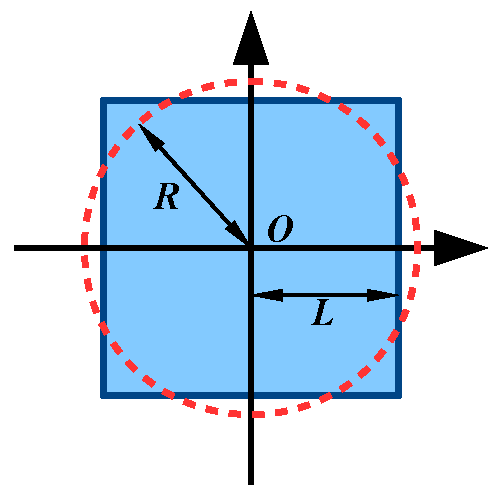
\includegraphics[width=.8 \linewidth, clip]{img/centralgravity.pdf}
			\caption{Illustration of benchmark for hydrostatic validation \label{fig:centralgravity}}
		\end{figure}
		\cref{fig:centralgravity}に、この妥当性確認で用いるベンチマークの概要図を示す。
		図のように2次元場で原点$O$を中心に長さ$2L$の正方形(青色実線)で粒子を初期配置し、中心重力下で時間発展させ十分な時間が経過すると、半径$R=\sqrt{4L^2/\pi}$(赤色点線)の表面形状に安定する。
		この時、
		\begin{itemize}
			\item 最も原点から遠い粒子の原点からの距離が\cref{eq:R}と一致するか
			\item 各粒子の圧力が\cref{eq:sp}と一致するか
		\end{itemize}
		を確認する。

	\subsection{水柱崩壊問題1 \label{subsec:dambreak1}}
		静水状態を解けることが確認できたら、次は流れがある状態でのベンチマークである。

		ここでは、MPS法の原論文\Cite{ref:mps}と同様に、水柱崩壊問題(あるいはダムブレーク問題)の先端位置を実験と比較する妥当性確認を考える。
		原論文で既に原始MPS法で妥当性確認されているため、本問題によって、OpenMPSの実装ないしは原始MPS法の後に導入された高精度手法の理論または実装の問題を知ることができる。

		\begin{figure} \centering
			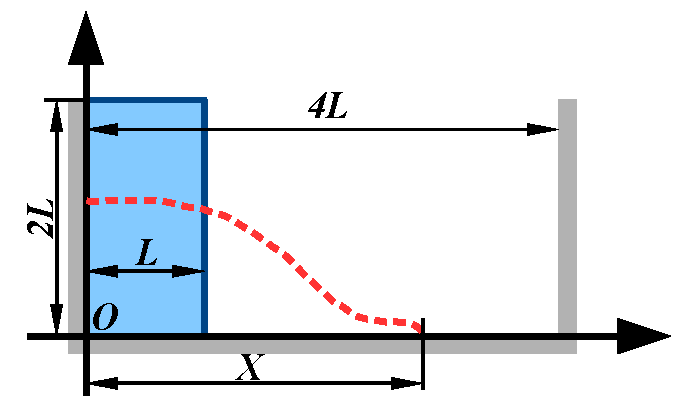
\includegraphics[width=\linewidth, clip]{img/dambreak1.pdf}
			\caption{Illustration of dambreak benchmark by Koshizuka \&Oka (1996) \label{fig:dambreak1}}
			\vspace*{-5mm}
		\end{figure}
		\cref{fig:dambreak1}に、この妥当性確認で用いるベンチマークの概要図を示す。
		図のように、幅$L$・高さ$2L$の水柱(青色実線)を、幅$4L$・高さ$2L$の水槽(灰色)に用意し、鉛直下向き重力下で時間発展させると、流体は重力とそれに伴って発生する圧力によって右方向へ流れる段波のようになる(赤色点線)。
		この時、各時刻におけるこの段波の先端座標$X$を計測し、その時系列(つまり波速)が実験と一致するかを確認する。

	\subsection{水柱崩壊問題2 \label{subsec:dambreak2}}
		\cref{subsec:dambreak1}の問題で波速(自由表面の形状の時系列)の妥当性確認をした後、最後に圧力の妥当性確認を実施する。

		\begin{figure} \centering
			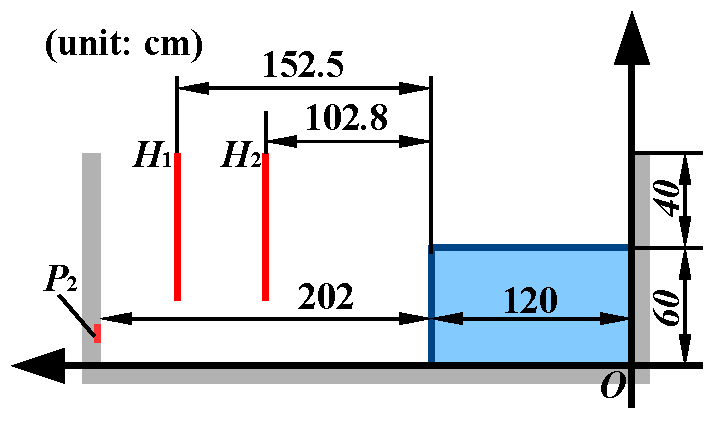
\includegraphics[width=\linewidth, clip]{img/dambreak2.pdf}
			\caption{Illustration of dambreak benchmark by Zhoou et al.(1999). A circle pressure gauge $P_2$, whose diameter is \SII{9}{cm}, is located \SII{16}{cm} from the bottom of the tank.\label{fig:dambreak2}}
		\end{figure}
		本ベンチマークは、Zhouら(1999)\Cite{ref:zhou1999}の実験を比較対象とする。
		\cref{fig:dambreak2}に、この妥当性確認で用いるベンチマークの概要図を示す。
		図のように、$H_1$および$H_2$に波高計があり、$P_2$で圧力を測定する。
		この時、各時刻におけるこれらの波高と圧力の時系列を、実験と比較し、一致するかを確認する。

\section{妥当性確認の結果 \label{sec:result}}
	\cref{sec:benchmark}のベンチマーク問題を用いて、DualSPHysicsとOpenMPSについて妥当性確認を実施した。
	その結果
	\begin{itemize}
		\item DualSPHysicsが静水状態で水深が増大する
		\item OpenMPSで流体が非物理的な加速をする
		\item OpenMPSで圧力擾乱が強い
	\end{itemize}
	という問題を発見した。詳細を以下に述べる。

	\subsection{静水圧 (DualSPHysics) \label{subsec:density}}
		\cref{subsec:centralgravity}の問題において$L=\SII{0.5}{m}$、初期粒子間距離\SII{0.008}{m}で粒子を初期配置し、DualSPHysicsで中心重力ベンチマークを実行した。
		DualSPHysicsの既定の設定から変更したものは以下の通りである(概ね、サンプルのダムブレーク問題と同様)。
		\begin{itemize}
			\item 重力加速度$g$:\SII{9.8}{m/s^2}
			\item 基準密度$\rho_0$:\SII{998}{kg/m^3}
			\item 粘性係数$\nu$: \SII{0.000894}{Pa.s}
			\item モデルパラメーター$c$の拡大係数:30倍
			\item カーネル関数:ウェンドランド形式
			\item カーネル半径$h$:初期粒子間距離の$0.91924 \sqrt{3}$倍
			\item 時間積分:シンプレック積分
			\item 粘性計算法:層流+SPS
			\item 粒子間相互作用の精度:倍精度
			\item $\delta$SPH法の係数:0.1
		\end{itemize}
		また、中心重力問題を解くためには、重力の方向を変更する必要があるため、基準となるソースコードを改変し実行した。

		\begin{figure*} \centering
			\begin{minipage}{.3 \linewidth} \centering
				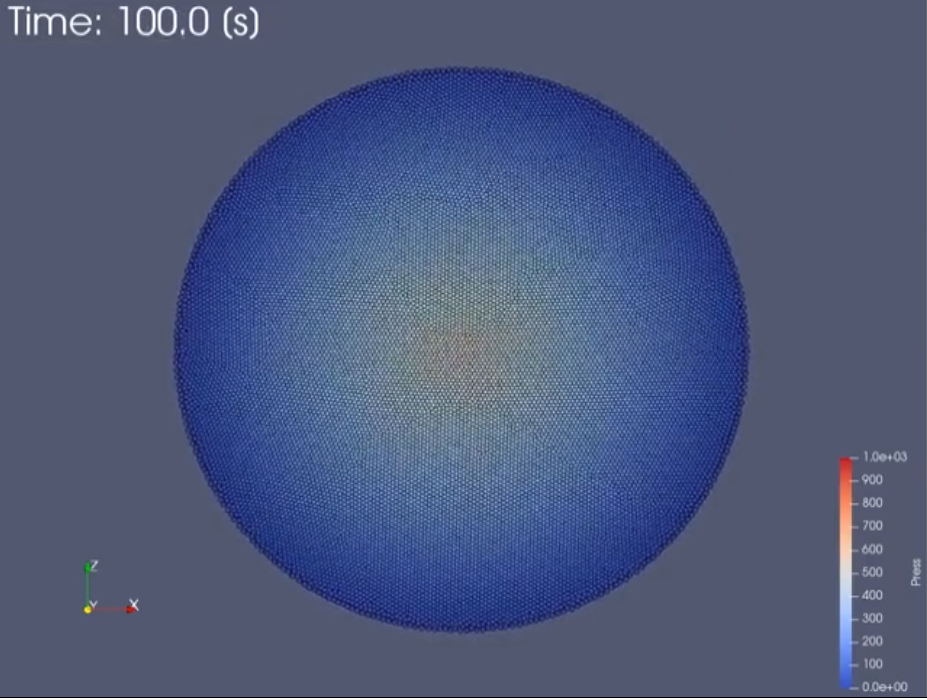
\includegraphics[clip, width=\linewidth]{img/dsph_snap_100.png}
				\subcaption{$t=\SII{100}{s}$}
			\end{minipage}
			\begin{minipage}{.3 \linewidth} \centering
				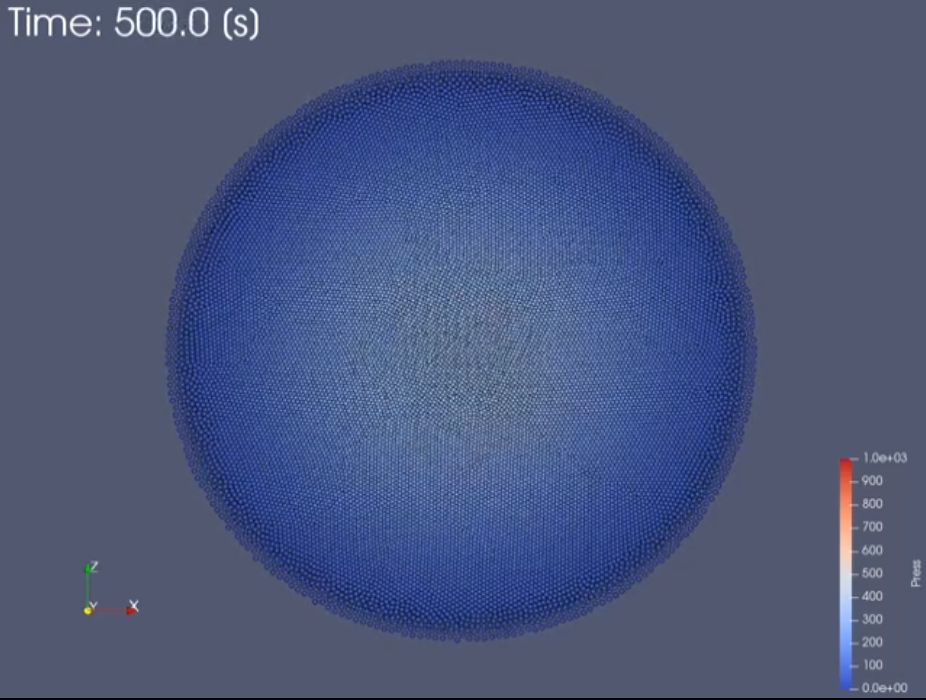
\includegraphics[clip, width=\linewidth]{img/dsph_snap_500.png}
				\subcaption{$t=\SII{500}{s}$}
			\end{minipage}
			\begin{minipage}{.3 \linewidth} \centering
				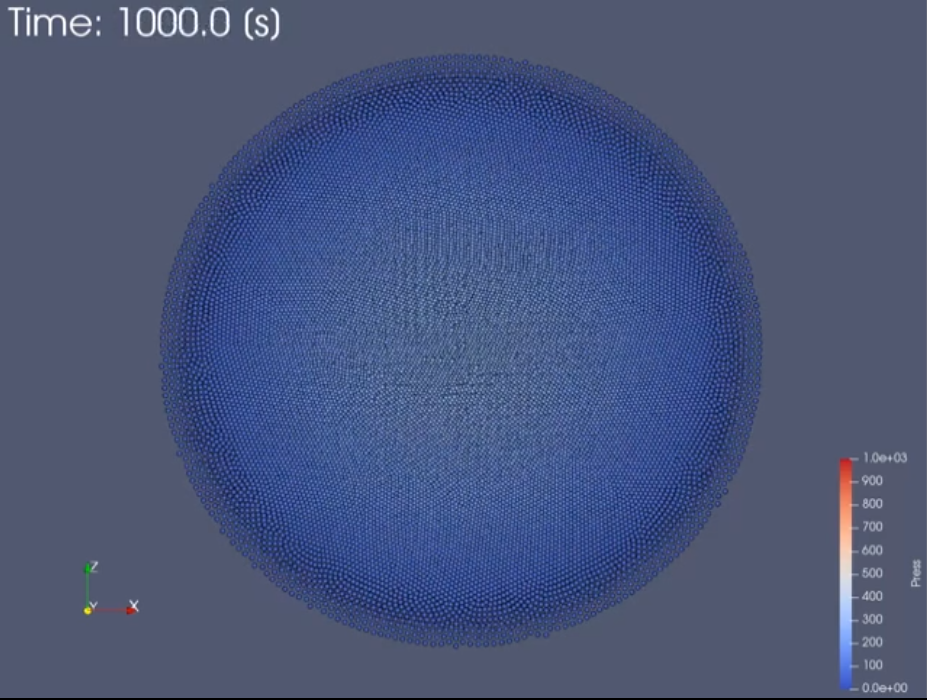
\includegraphics[clip, width=\linewidth]{img/dsph_snap_1000.png}
				\subcaption{$t=\SII{1000}{s}$}
			\end{minipage}
			\caption{Result of the Central Gravity Benchmark with DualSPHysics \label{fig:dsph}}
		\end{figure*}
		\cref{fig:dsph}に結果を示す。
		このように、時間が経過すると中心から自由表面までの距離が増大し、圧力が低下してしまう結果となった。
		この結果は明らかに非物理的挙動であり、自由表面付近を拡大してみると、粒子間の距離が増大している様子が見て取れた。

		この原因は、密度計算法の問題であると考えられる。
		DualSPHysicsでは、密度の計算を\cref{eq:rho_sph}の形ではなく、\cref{eq:drho}のような時間微分形式を時間発展させる手法を適用している。
		\begin{equation}
			\frac{\mathrm{D} \rho }{\mathrm{D} t} = \sum_{j \neq i} m_j \left( \mathbf{u}_j - \mathbf{u}_i \right) \cdot \mathbf{\nabla} W_{ji} \label{eq:drho}
		\end{equation}
		本来であれば、完全に静水状態であれば流速$\mathbf{u}$は常に0のため密度は時間によって変化しない。
		しかし、数値誤差などによってわずかに値を持った結果、その誤差が蓄積し密度が徐々に増減した結果、\cref{eq:wcsph}の圧力分布に勾配が生まれ、結果的に粒子が存在しない空間へ粒子が移動してしまう。

		\begin{figure} \centering
			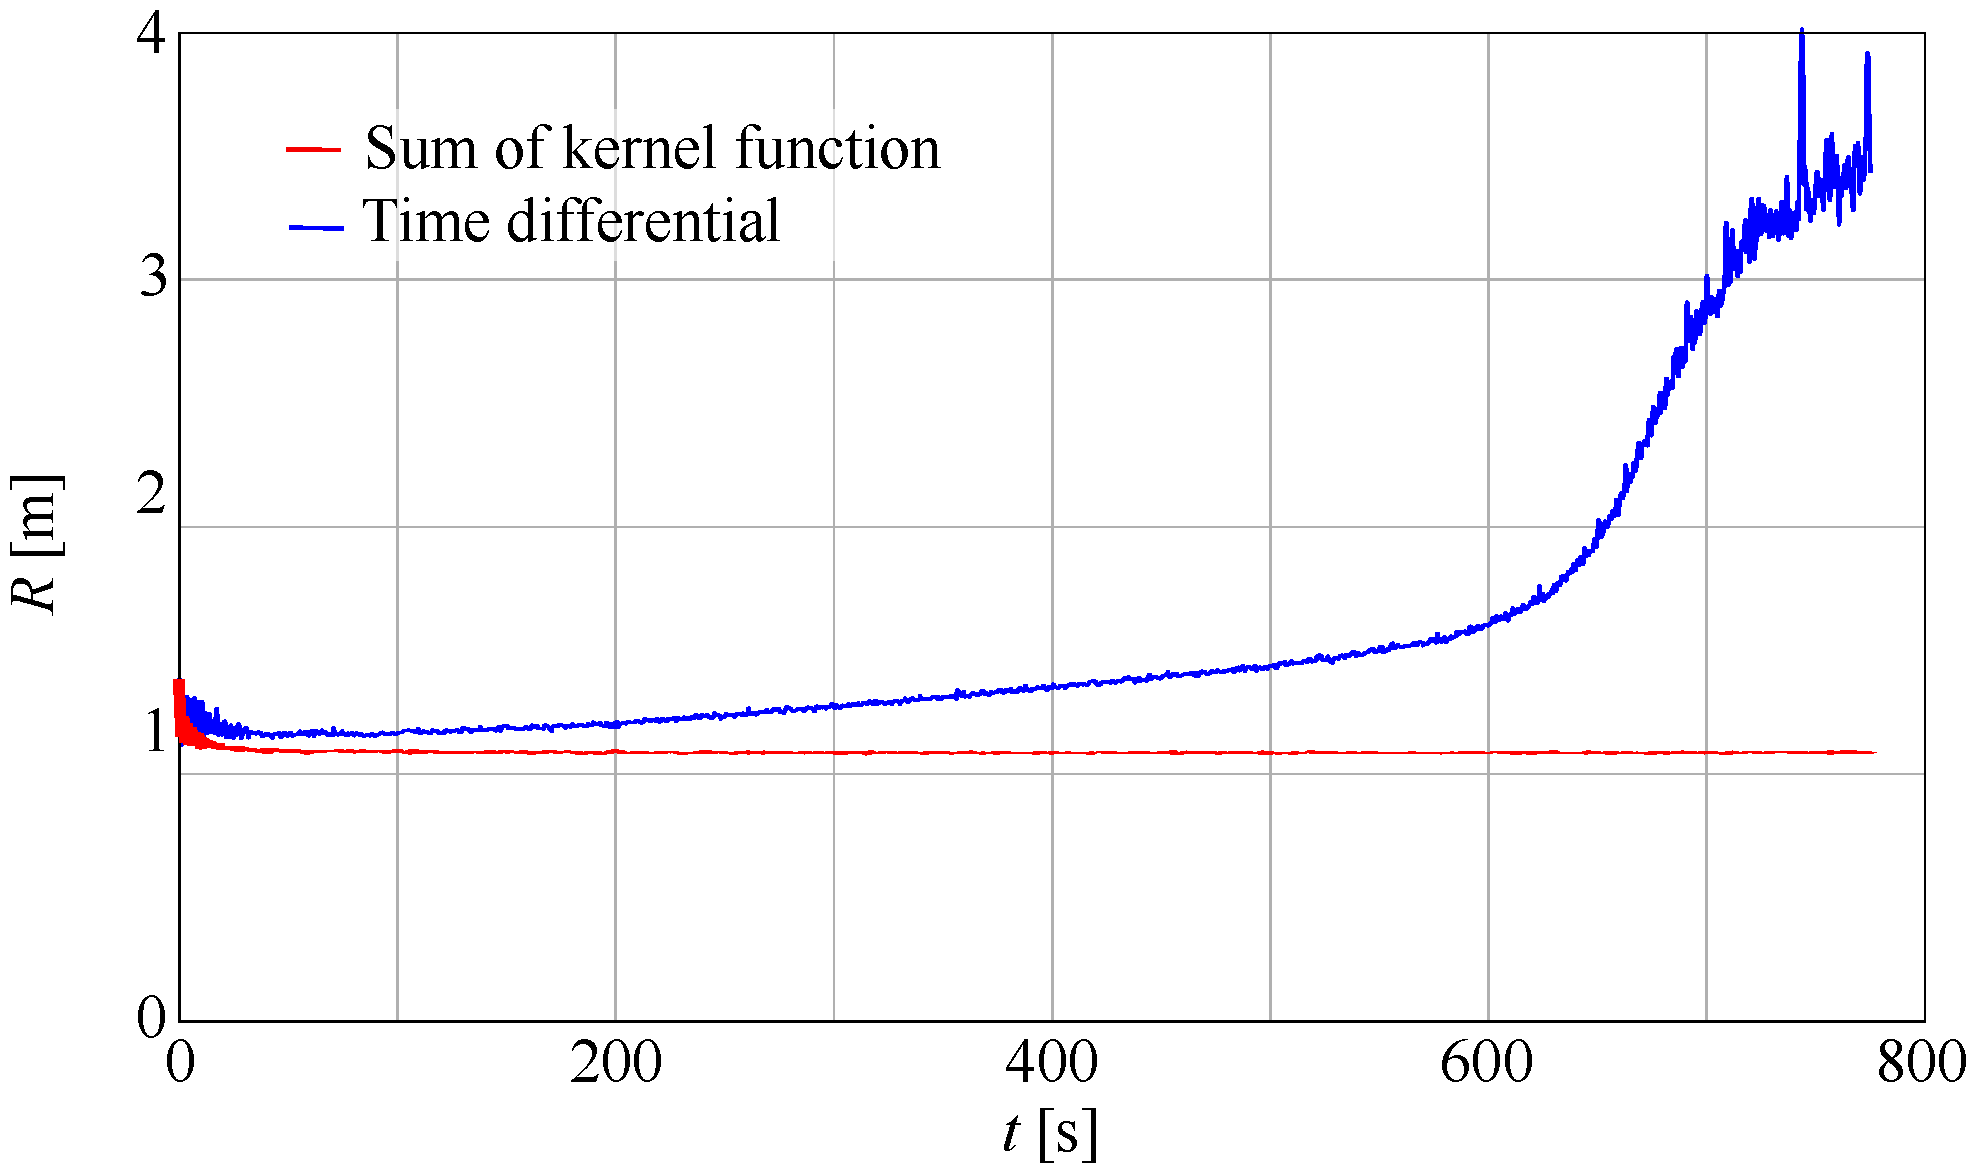
\includegraphics[clip, width=\linewidth]{img/time-radius.pdf}
			\caption{Difference by density formulation, with self-made WCSPH program \label{fig:rho_sum}}
		\end{figure}
		実際に、WCSPH法を簡易的に手元で実装し比較したところ、\cref{fig:rho_sum}のように、\cref{eq:rho_sph}のカーネル関数の和の形であれば原点から自由表面の距離$R$は時間経過でも変化しないが、
		\cref{eq:drho}の時間微分形に変えた場合は$R$が増大する現象を確認した。

		このように、DualSPHysicsでは静水圧問題が解けていないことが判明したため、以降の妥当性確認はOpenMPSでのみ実施した。

	\subsection{静水圧 (OpenMPS) \label{subsec:gc}}
		\cref{subsec:centralgravity}の問題において$L=\SII{0.5}{m}$、初期粒子間距離\SII{0.005}{m}で粒子を初期配置し、OpenMPSで中心重力ベンチマークを実行した。
		DualSPHysicsと同様に、重力方向を変更するために改変が必要だったため、改変を加えたバージョン(コミットハッシュ2f1313e)を対象とする。

		\begin{figure*} \centering
			\begin{minipage}{.3 \linewidth} \centering
				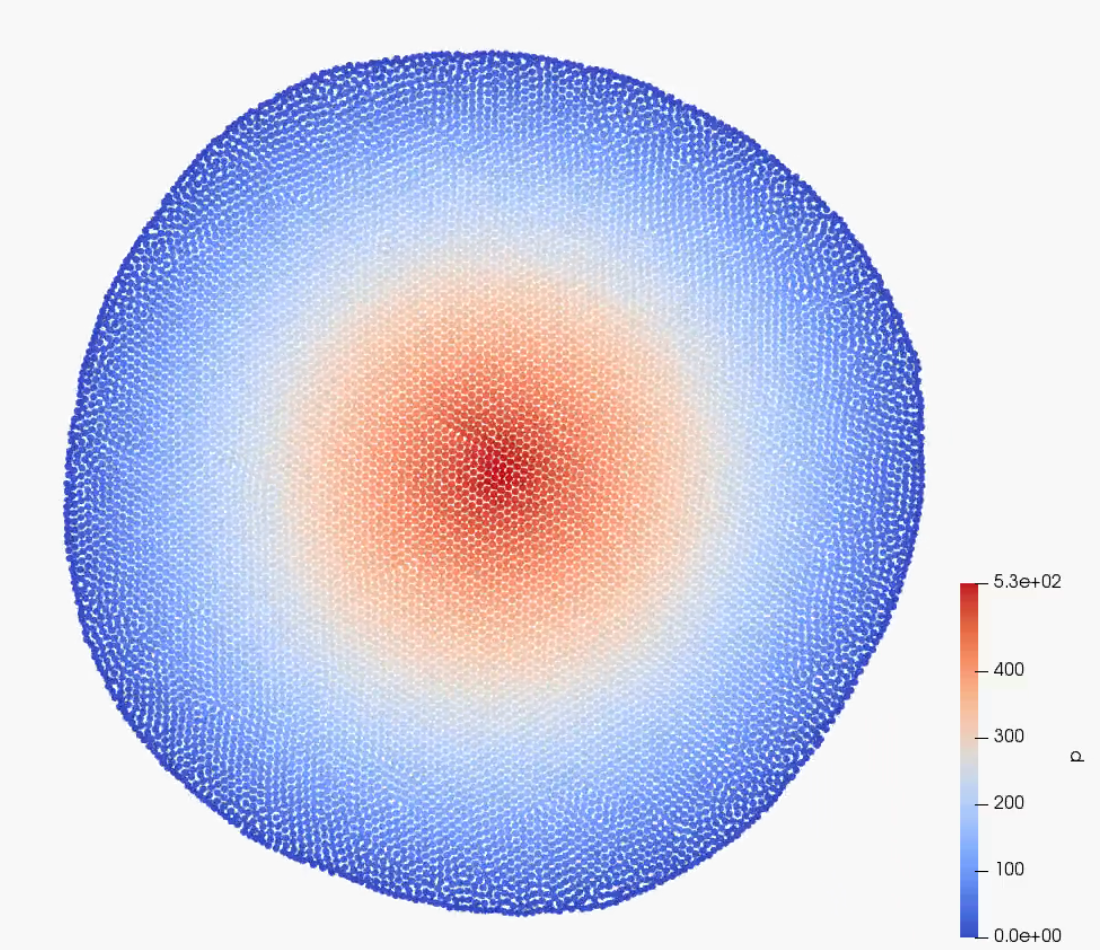
\includegraphics[clip, width=\linewidth]{img/mpsgc_10.png}
				\subcaption{$t=\SII{10}{s}$}
			\end{minipage}
			\begin{minipage}{.3 \linewidth} \centering
				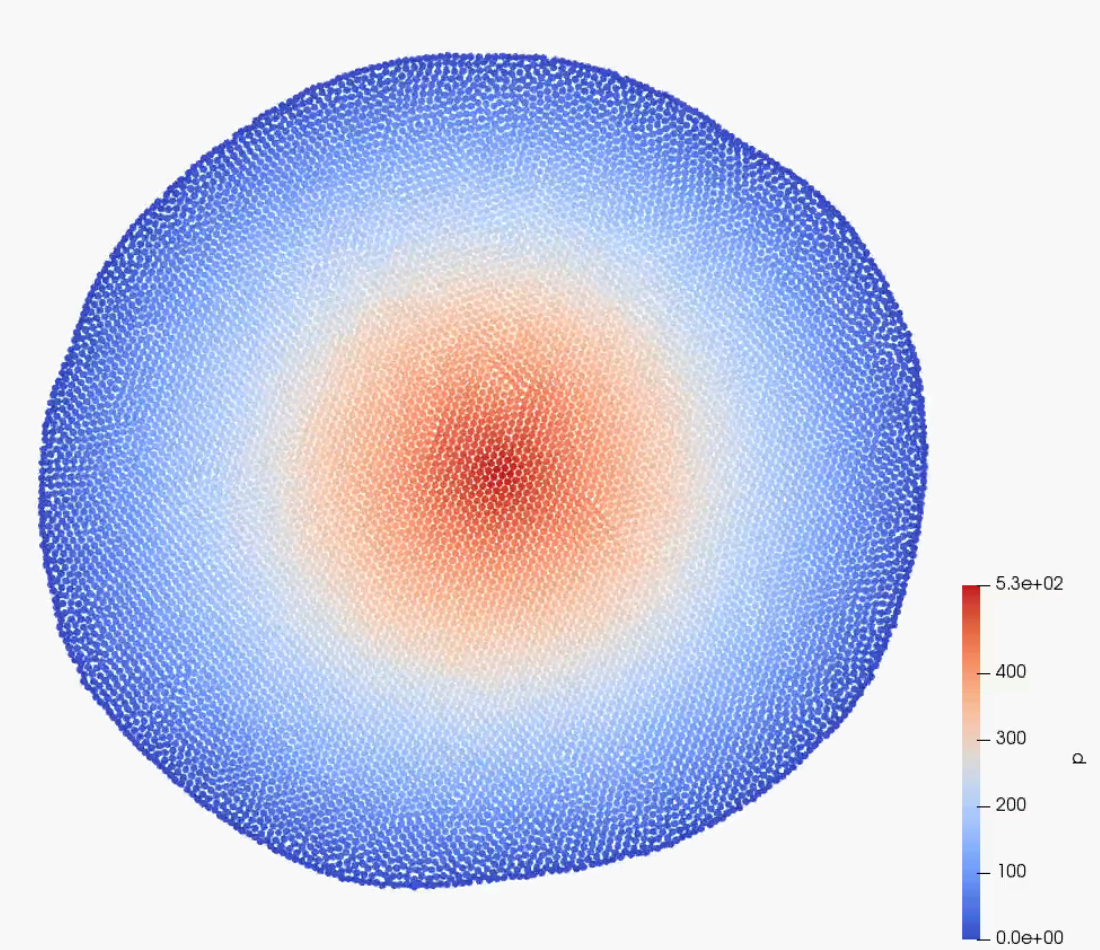
\includegraphics[clip, width=\linewidth]{img/mpsgc_30.png}
				\subcaption{$t=\SII{30}{s}$}
			\end{minipage}
			\begin{minipage}{.3 \linewidth} \centering
				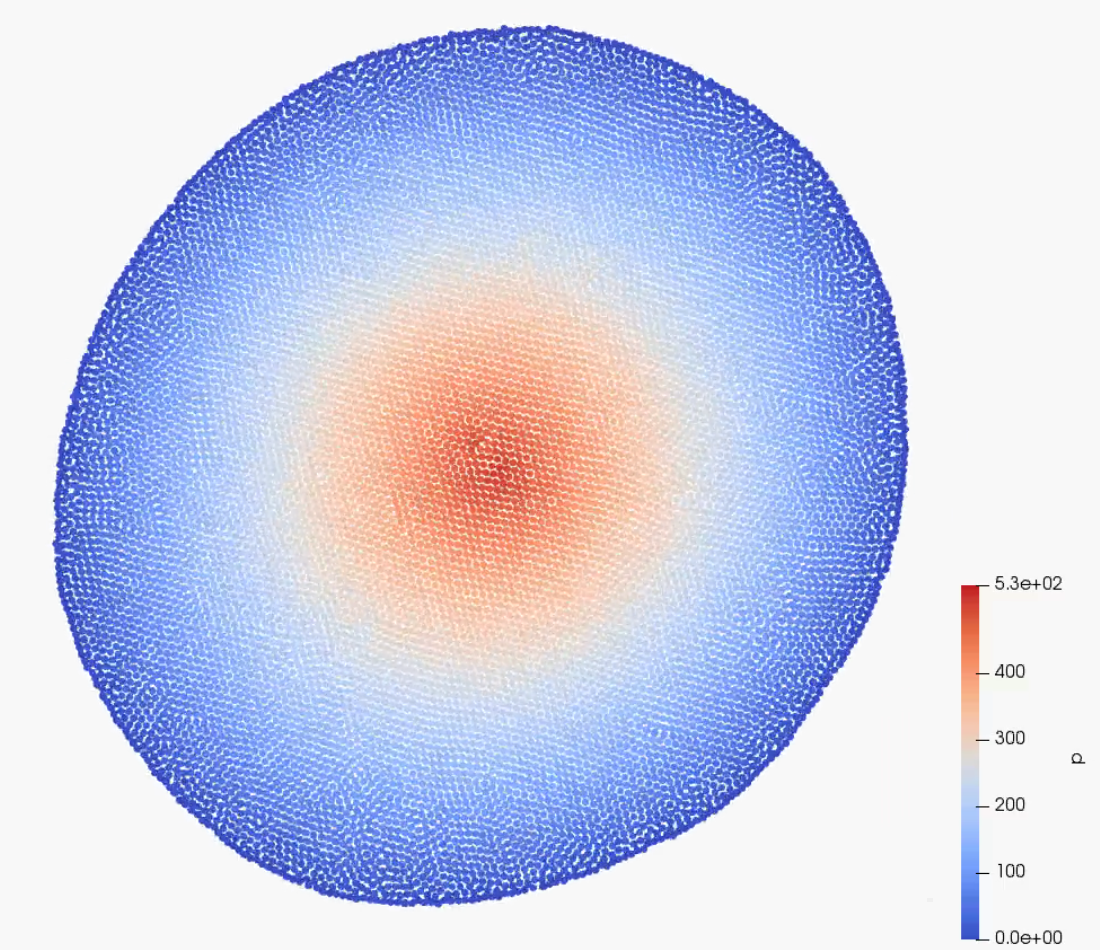
\includegraphics[clip, width=\linewidth]{img/mpsgc_40.png}
				\subcaption{$t=\SII{40}{s}$}
			\end{minipage}
			\caption{Result of the Central Gravity Benchmark with OpenMPS (with GC) \label{fig:mps_gc}}
		\end{figure*}
		\cref{fig:dsph}に結果を示す。
		このように、時間が経過しても自由表面が安定せず、水面が非物理的な動揺が続いてしまう結果となった。

		この原因は高精度粒子法のうち勾配修正(GC)法\Cite{ref:Khayyer2011}にあった。勾配修正法では、勾配モデルを\cref{eq:grad_mps}から変更し、\cref{eq:gc}で計算する。
		\begin{equation}
			\mathbf{\nabla} \phi_i = \frac{D}{n_0} \sum_{j \neq i} \frac{\phi_i - \phi_i}{\left| \mathbf{r}_{ji} \right|} \frac{{C_i}^{-1} \mathbf{r}_{ji}}{\left| \mathbf{r}_{ji} \right|} w_{ji} \label{eq:gc}
		\end{equation}
		ここで$C_i$は、\cref{eq:cmatrix}で計算される勾配修正行列である。
		\begin{equation}
			C_i = \frac{D}{n_0} \sum_{j \neq i} \frac{\mathbf{r}_{ji} \otimes \mathbf{r}_{ji}}{{\left| \mathbf{r}_{ji} \right|}^2} w_{ji} \label{eq:cmatrix}
		\end{equation}
		これにより、近傍粒子分布によらず1次精度になるのだが、$C_i$(の逆行列)は近傍粒子分布によって変化するため、必ずしも$i$粒子と$j$粒子で同じではない。
		つまり、勾配修正行列で補正された勾配モデルで圧力勾配を計算すると、粒子間の相互作用が非対称となり、非物理的な運動量が発生してしまっていたことで、静水状態になることができていなかったと考えられる。
		
		\begin{figure} \centering
			\begin{minipage}{\linewidth} \centering
				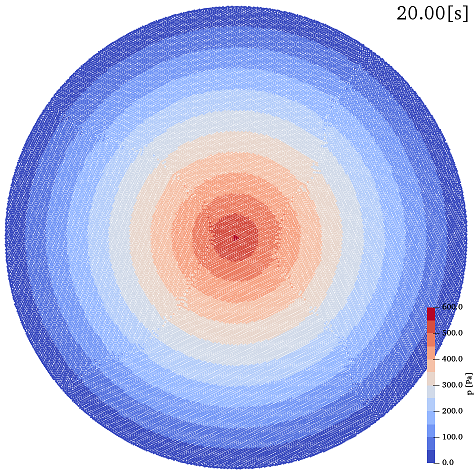
\includegraphics[clip, width=\linewidth]{img/mps_nogc_snap.png}
				\subcaption{Snapshot ($t = \SII{20}{s} $)}
			\end{minipage}
			\begin{minipage}{\linewidth} \centering
				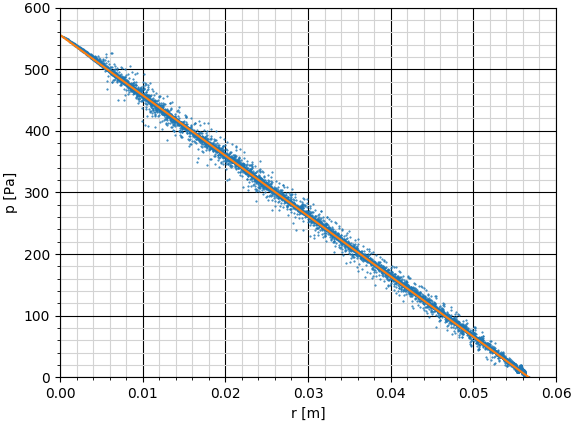
\includegraphics[clip, width=\linewidth]{img/mps_nogc_p.png}
				\subcaption{Pressure distribution. Orange line represent hydrostatic pressure Eq.~(\ref{eq:sp})}
			\end{minipage}
			\caption{Result of the Central Gravity Benchmark without GC method \label{fig:nogc}}
		\end{figure}
		実際に勾配修正法を無効化したOpenMPS(コミットハッシュbaa36a9)で再度ベンチマークを実行したところ\cref{fig:nogc}のように、円形に安定し、圧力分布も理論通りとなった。

		以上より、OpenMPSにおいては、勾配修正法に問題があり静水圧がうまく解けなかったが、勾配修正法を無効化することで解決し、静水圧の妥当性確認ができた。

	\subsection{自由表面形状 \label{subsec:dambreak1_result}}
		\cref{subsec:dambreak1}の問題において$L=\SII{0.146}{m}$、初期粒子間距離を\SII{0.008}{m}で初期配置し、OpenMPSで水柱崩壊ベンチマークを実行した。
		この形状設定は、原始MPS法での計算\Cite{ref:mps}と同じものである。
		この時のOpenMPSのバージョンは、 \cref{subsec:gc}の勾配修正法を無効化したバージョン(コミットハッシュbaa36a9)を使用した。

		\begin{figure} \centering
			\begin{minipage}{\linewidth} \centering
				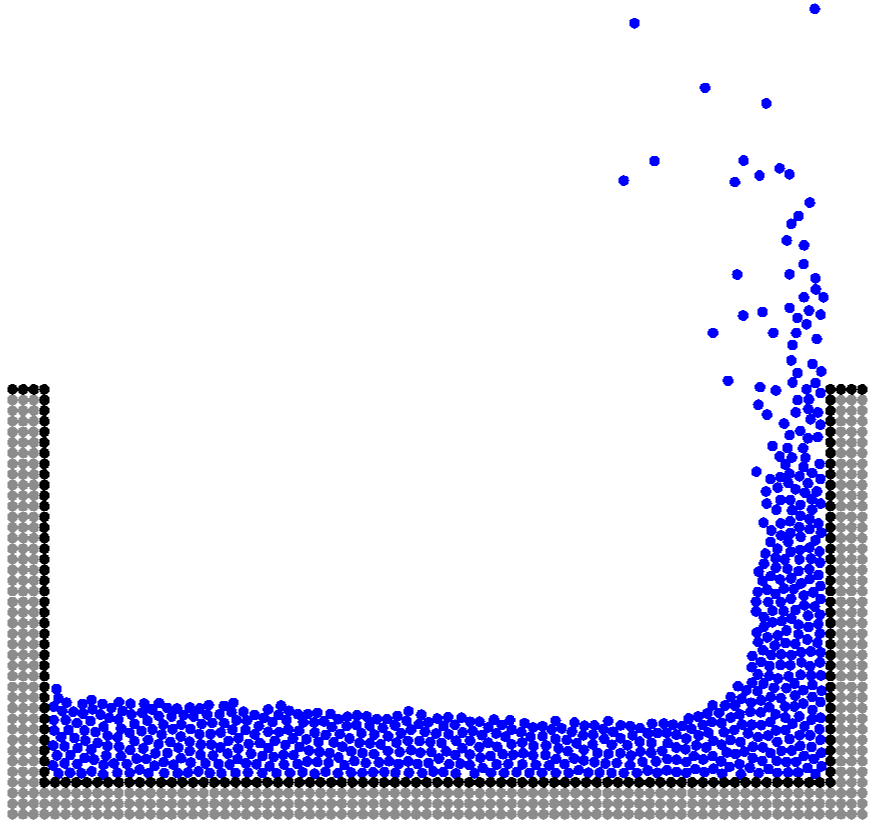
\includegraphics[clip, width=\linewidth]{img/dambreak1_snap.png}
				\subcaption{Snapshot ($t=\SII{5}{s}$)}
			\end{minipage}
			\begin{minipage}{\linewidth} \centering
				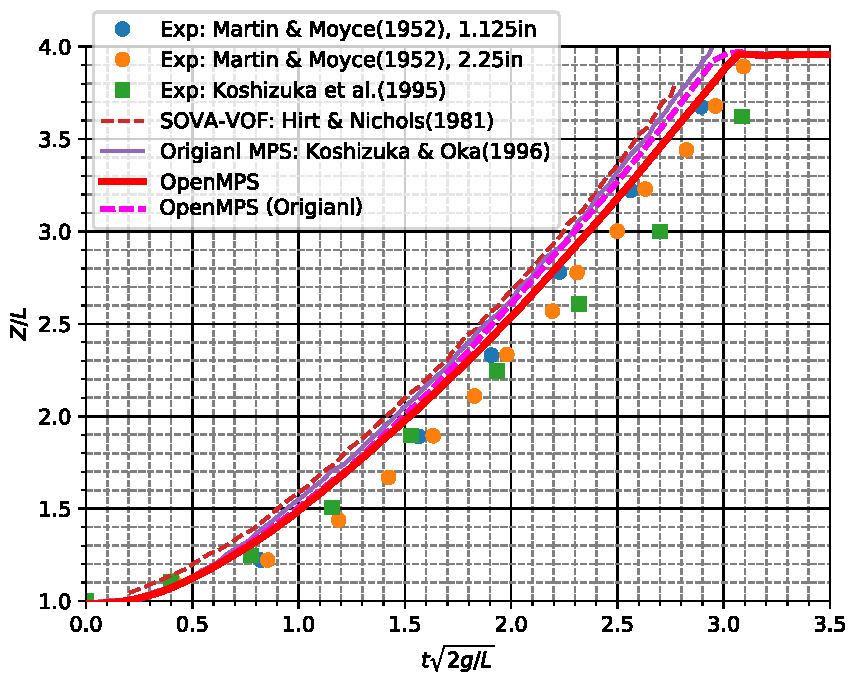
\includegraphics[clip, width=\linewidth]{img/koshizuka_oka_1996.pdf}
				\subcaption{Comparison with experimental and other computed result}
			\end{minipage}
			\caption{Result of the Koshizuka\&Oka(1996) Dambreak Benchmark \label{fig:result_dambreak1}}
		\end{figure}
		\cref{fig:result_dambreak1}にベンチマークの実行結果を示す。
		図のように、通常のOpenMPSは、原始MPS法に比べ実験値に近い結果を示した。
		OpenMPSと原始MPS法との違いは高精度粒子法(MPS-HS-HL-ECS-DS)の有無であるため、高精度粒子法により、実験値に近い結果になったと考えられる。
		高精度粒子法の効果を確かめるため、OpenMPSで高精度粒子法をすべて無効化し原始MPS法と同等にした時の計算も実施し、図中に合わせた。
		結果、確かに、高精度粒子法を切ると、より原論文に近い結果を得ることができた。

	\subsection{水深と圧力 \label{subsec:spp}}
		\cref{subsec:dambreak2}において、初期粒子間距離を\SII{0.002}{m}で初期配置し、OpenMPSで水柱崩壊ベンチマークを実行した。
		この時のOpenMPSのバージョンは\cref{subsec:dambreak1_result}と同じ(コミットハッシュbaa36a9)を使用した。

		\begin{figure*} \centering
			\begin{minipage}{.7 \linewidth} \centering
				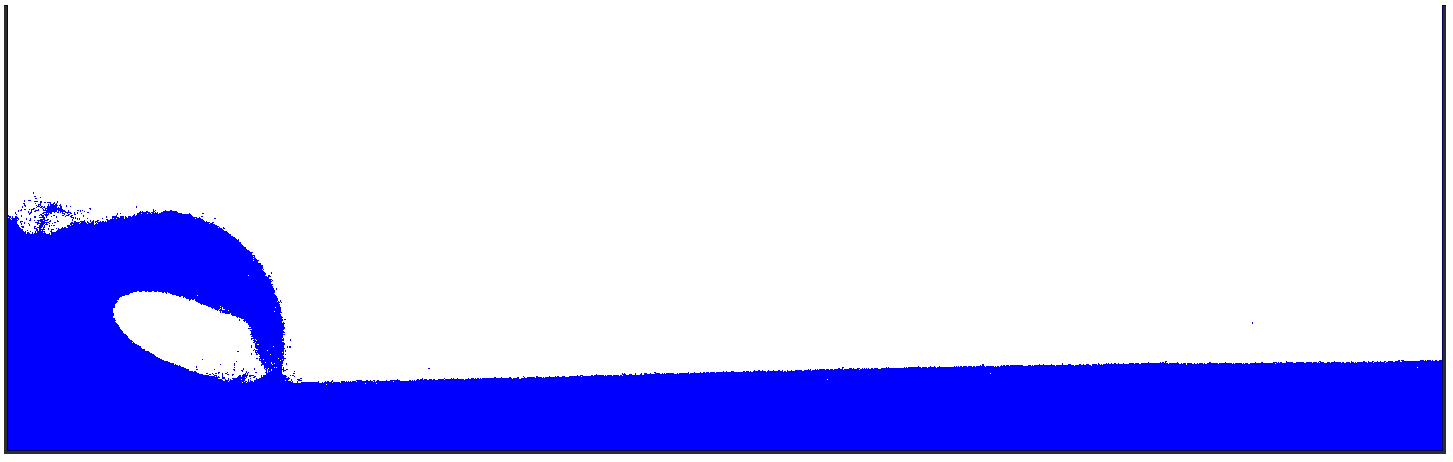
\includegraphics[clip, width=\linewidth]{img/dambreak2_snap.png}
				\subcaption{Snapshot ($t=\SII{1.5}{s}$)}
			\end{minipage}
			\begin{minipage}{.3 \linewidth} \centering
				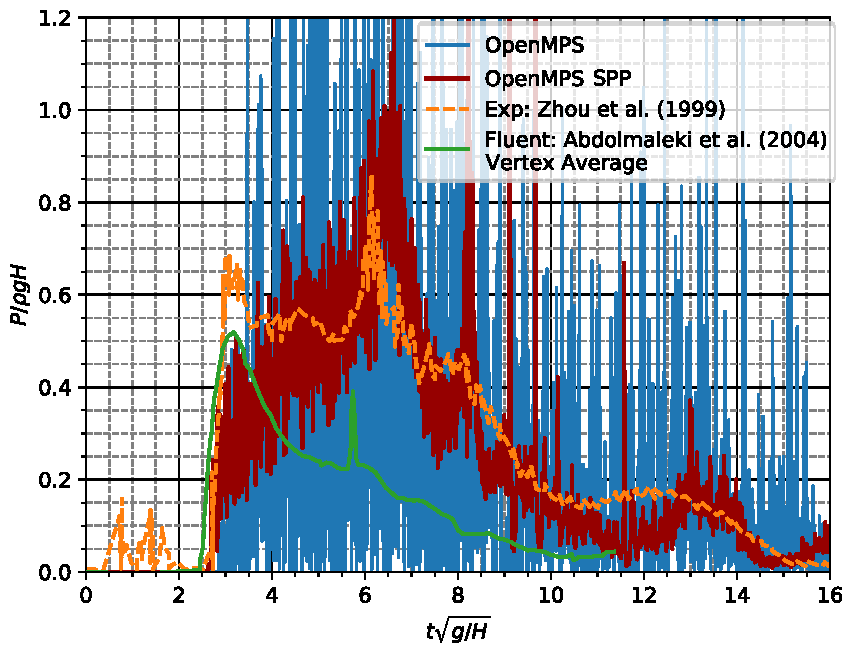
\includegraphics[clip, width=\linewidth]{img/zhouetal1999_p2_2mm.pdf}
				\subcaption{Pressure at $P_2$ \label{fig:dambreak2_p}}
			\end{minipage}
			\begin{minipage}{.3 \linewidth} \centering
				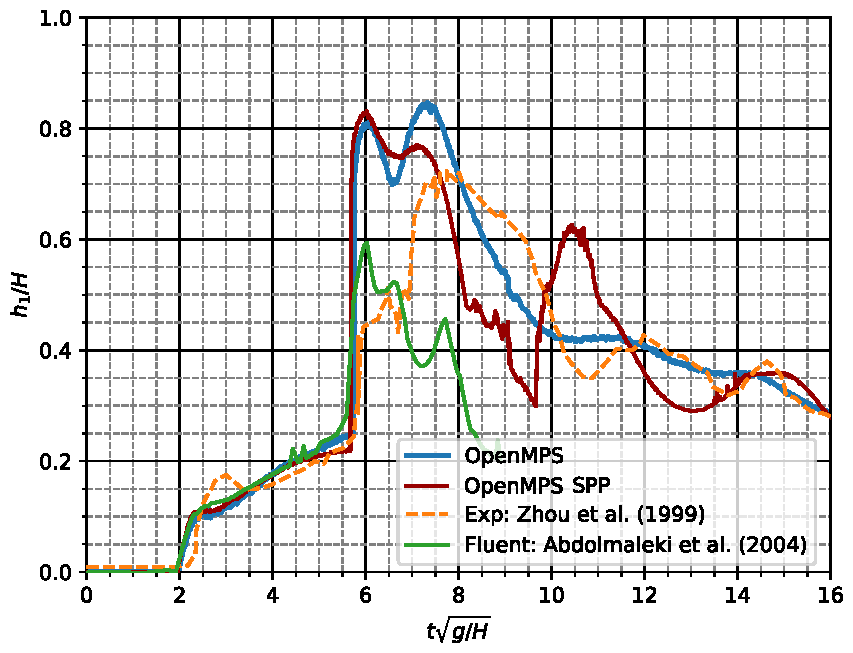
\includegraphics[clip, width=\linewidth]{img/zhouetal1999_h1_2mm.pdf}
				\subcaption{Water depth at $H_1$ \label{fig:dambreak2_h1}}
			\end{minipage}
			\begin{minipage}{.3 \linewidth} \centering
				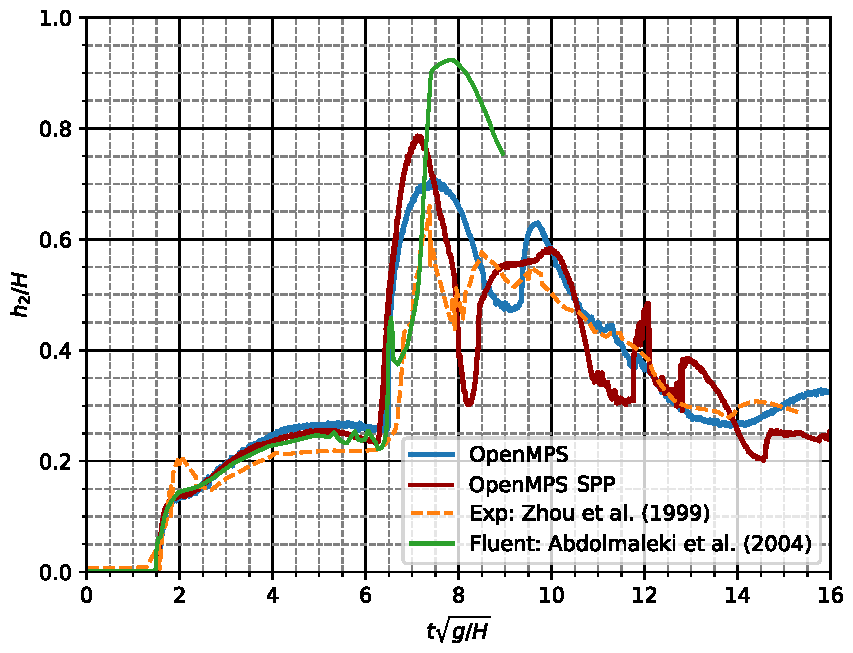
\includegraphics[clip, width=\linewidth]{img/zhouetal1999_h2_2mm.pdf}
				\subcaption{Water depth at $H_2$ \label{fig:dambreak2_h2}}
			\end{minipage}
			\caption{Result of the Zhou et al.(1999) Dambreak Benchmark \label{fig:result_dambreak2}}
		\end{figure*}
		\cref{fig:result_dambreak2}に実行結果を示す。
		\cref{fig:dambreak2_h1,fig:dambreak2_h2}のように水深については\SII{6}{s}あたりの立ち上がり(反射波の到達)時刻が実験とほぼ一致し、その後の結果もFluentの結果に比べ実験に近い値を得ることができた。

		一方、\cref{fig:dambreak2_p}の通り、圧力については擾乱がひどく、まともに評価することができていなかった。		
		粒子法、特に射影法型の陰的粒子法では張力不安定性(tensile instability)の問題で圧力に擾乱があることはあるが、これほどの擾乱は今後の利用に支障をきたす。
		原因を探ったところ、計算中に粒子が移動した時に生じる僅かな空隙によって流体内部に自由表面として判定される粒子がいくつか発生し、それが原因となっていた。
		
		そのような不自然な空隙を抑えるには、高精度粒子法のうち自由表面仮想粒子(SPP)法\Cite{ref:Tsuruta2015}が有効であることが知られている。
		そこでOpenMPSに新たにSPP法を実装し比較してみたところ(\cref{fig:dambreak2_p}の赤色)、圧力擾乱がかなり低減され、概ね実験値に近い値となった。

\section{結論と今後の課題}
	本研究では、粒子法FLOSSの発展に寄与するため、DualSPHysicsとOpenMPSという2つのソフトウェアについて妥当性確認を実施した。
	ベンチマークでの比較対象としたのは、静水圧・自由表面形状・圧力という基本的な物理量で、中心重力問題と水柱崩壊問題を用いた。
	結果、DualSPHysicsでは密度の計算法がカーネル和型ではなく時間微分の発展型であることにより、誤差蓄積で静水状態で自由表面が膨らんでしまう問題を発見した。
	また、OpenMPSでは、実装されている勾配修正法が非物理的な運動量の湧き出しを誘引していたことと、流体内部の空隙により過大な圧力擾乱が生じていた問題を発見した。
	これらについては、勾配修正法の無効化とSPP法を導入することで改善され、OpenMPSの改善に寄与することができた。

	今後については、まずDualSPHysicsでの密度計算式を実際にカーネル和型に変更し、もし効果が確認できれば、開発元へPull Requestを提出したい。
	OpenMPSについては、勾配修正法の改善を目指したい。
	今回は勾配修正法を無効化することとしたが、高精度粒子法である以上は導入されているほうが精度が良いはずである。
	そのため、引き続き調査し、実装上のバグや理論との乖離などがないかを確かめ、もしない場合は理論的な改善も検討したい。
	更に、関数単体での試験などVerificationが不足しているため、それらの開発提案をすることで、デバッグや精度改善に貢献したいと考えている。
	そして、今回用いたベンチマークはいずれも仮想的な問題であったことから、さらにベンチマークの種類を増やし、より現実的な条件での妥当性確認を実施したい。
	例えば、強制振動水槽による液面動揺問題(スロッシング)や、海岸・海洋工学に欠かせない造波・消波といった境界条件を試す問題が望まれる。

	今後も、このような活動を継続しその成果を報告することで、今回対象としたDualSPHysicsとOpenMPSを含めた粒子法FLOSSや広くオープンCAEの改善・利用を促進し、安全な人類社会の実現に貢献していきたいと考えている。

\section*{参考文献}

\begin{enumerate}
    \item プロメテック・ソフトウェア:「Particleworks」\url{https://www.particleworks.com/} \label{ref:particleworks}
    \item Dassault Systèmes: ``Abaqus/Explicit'' \url{https://www.3ds.com/products-services/simulia/products/abaqus/abaqusexplicit/} \label{ref:abaqus}
    \item 富士テクニカルリサーチ:「MPS-RYUJIN」\url{https://www.ftr.co.jp/solution/software/ryujin/} \label{ref:ryujin}
	\item ``DualSPHysics'' \url{https://dual.sphysics.org/} \label{ref:dualsphysics}
	\item Gingold R.A., Monaghan J.J. (1977): ``Smoothed particle hydrodynamics: theory and application to non-spherical stars'', Mon. Not. R. Astron. Soc. 181, pp.375–389. \label{ref:sph1}
	\item Lucy L.B. (1977): ``A numerical approach to the testing of the fission hypothesis'', Astron. J. 82, pp.1013–1024. \label{ref:sph2}
	\item Monaghan J.J. (1994): ``Simulating free surface flows with SPH'', J.Comput. Phy., Vol.110, pp.399-406. \label{ref:wcsph}
	\item ``OpenMPS'' \url{https://openmps.github.io/} \label{ref:openmps}
	\item Koshizuka, S. and Oka, Y.(1996): ``Moving particle semi-implicit method for fragmentation of incompressible fluid'', Nuclear Science and Engineering, 123, pp.421-434. \label{ref:mps}
	\item 越塚誠一 (2005): 「計算力学レクチャーシリーズ 粒子法」、丸善。 \label{ref:koshizuka2005}
	\item 後藤人志 (2018): 「粒子法 連続体・混相流・粒状体のための計算科学」、森北出版。 \label{ref:gotoh2018}
	\item Khayyer A, Gotoh H (2009): ``Modified moving particle semi-implicit methods for the prediction of 2D wave impact pressure'', Coast Eng, 56, pp.419–440. \label{ref:Khayyer2009}
	\item Khayyer A, Gotoh H (2010): ``A higher order laplacian model for enhancement and stabilization of pressure calculation by the MPS method", Appl Ocean Res, 32(1), pp.124–131. \label{ref:Khayyer2010}
	\item Khayyer A, Gotoh H (2011): ``Enhancement of stability and accuracy of the moving particle semi-implicit method'', J Comput Phys, 230, pp.3093–3118. \label{ref:Khayyer2011}
	\item Tsuruta N, Khayyer A, Gotoh H (2013): ``A short note on dynamic stabilization of moving particle semi-implicit method'', Comput Fluids, 82, pp.158–164. \label{ref:Tsuruta2013}
	\item Tsuruta N, Khayyer A, Gotoh H (2015): ``Space potential particles to enhance the stability of projection-based particle methods'', Int J Comput Fluid Dyn, 29(1), pp.100–119. \label{ref:Tsuruta2015}
	\item Gotoh H, Khayyer A (2016) ``Current achievements and future perspectives for projection-based particle methods with applications in ocean engineering'',  J Ocean Eng Mar Energy, 2. \label{ref:gotoh2016}
	\item Zhou Z.Q., De Kat J.O., Buchner B. (1999): ``A nonlinear 3-D approach to simulate GREEN WATER dynamics on deck'', In Proceedings 7th Intern. Conf. on Numerical Ship Hydrodynamics. \label{ref:zhou1999}
\end{enumerate}

\end{document}
